\documentclass[aps, pre, reprint]{revtex4-1}
\usepackage{graphicx}
\usepackage{color}
\usepackage{amssymb}
\usepackage{afterpage}
\usepackage{amsmath}
\usepackage{tabularx}
\usepackage{bm}
\usepackage{hyperref}
\usepackage{ltxtable}
\usepackage{natbib} 
\usepackage{longtable}
%\usepackage{caption}
%\captionsetup[figure]{font=small,labelfont=normalsize}
\usepackage{float}
\newcommand{\be}{\begin{equation}}
\newcommand{\ee}{\end{equation}} 
\newcommand{\bes}{\begin{equation*}}
\newcommand{\ees}{\end{equation*}} 
\newcommand{\bea}{\begin{eqnarray}}
\newcommand{\eea}{\end{eqnarray}}


\usepackage[usenames,dvipsnames]{xcolor}
\hypersetup{
colorlinks,
citecolor=blue,
filecolor=blue,
linkcolor=blue,
urlcolor=blue}

\begin{document}
\title{Chaos control using deep reinforcement learning}

\author{Sumit Vashishtha}
\email{vash.sumit@gmail.com}
\affiliation{Florida Atlantic University}

\author{Siddhartha Verma}
\email{vermas@fau.edu}
\affiliation{Florida Atlantic University}

\date{\today}

\begin{abstract}
    {We use deep reinforcement learning to illustrate its utility in controlling chaotic systems. The report also serves as a brief review of different theoretical concepts that drive deep reinforcement learning as well as a few applications of the same in fields as diverse as Computer Vision,  health care, amongst others.}
 
\end{abstract}
\pacs{47.27.ef, 47.27.em, 47.27.ep}
% 47.27.te Turbulent convective heat transfer
% 47.55.P- Buoyancy-driven flows; convection

\maketitle
\section{Introduction}
\label{sec:intro}

Reinforcement learning is the third paradigm of machine learning; supervised and unsupervised            learning being the other two. Unlike the latter two approaches reinforcement learning is much more  focused on goal-directed learning from interaction with the environment. Reinforcement learning is learning what to do—how to map situations to actions—so as to maximize a numerical reward signal. The learner is not told which actions to take, but instead must discover which actions yield the most reward by trying them. Since it first appeared in the 1950s, reinforcement learning has produced many different applications over the past decades. However, its revolution started a couple of years ago when the researchers from DeepMind (an English startup) presented to the world some pretty interesting ideas~\cite{silver2016mastering}. DeepMind presented a system that was able to play any Atari game without prior knowledge or
experience. With the help of raw pixels as only inputs, this system outperformed the world champion of the GO game. Since then Reinforcement learning has burgeoned its presence ~\cite{barto2017some} in different fields ranging from playing games to finance.\\

A reinforcement learning problem consists of five major elements- state space A, action space S, environment , reward (r), policy space ($\Pi$). An RL agent interacts with an environment over time. At each time step $t$, the agent receives a state $s_t$ of environment from S, and and selects an action $a_t$
from A following a policy $\pi(a_t|s_t)$. This action transitions the agent to another state $s_{t+1}$ after following a model of the environment. The agent is rewarded with a reward $r_t$ for this transition. In  an episodic problem , this process continues until the agent reaches a terminal state and then it restarts. The return is the discounted, accumulated reward with the discount factor $\gamma$ which lies between $0$ and $1$. This discount factor increases the importance of present reward as compared to those in future. The cumulative reward, $R(a_t|s_t)$, is then given by,
\be
R(a_t|s_t) = \sum_{k=0}^{\infty} \gamma^{k}r_{t+k}
\ee
The goal of the RL agent is to maximize this cumulative reward by discovering an optimal policy $\Pi^{*}$. This entire process is further illustrated in Fig.\ref{fig:fig_1}.  There are different methods of attaining this (discussed later). Deep RL is the merging of deep neural networks with reinforcement learning algorithms in order to aid the learning process. Such factors as representation learning, generality, expressiveness and flexibility of deep neural networks aid in tremendously in the learning of RL algorithms. Deep RL is the recent buzzword in all of AI and thus deserves a good understanding. This report discusses different concepts related to Deep RL. \\

\begin{figure}[ht!]
\begin{center}
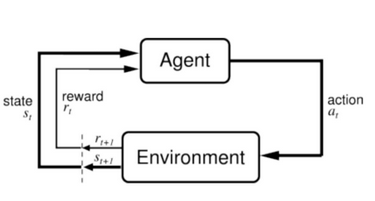
\includegraphics[scale=0.4]{rl_pic.png}
\end{center}
\caption { Schematic of a typical RL problem}
\label{fig:fig_1} 
\end{figure}
     

The outline of this report is as follows: In Sec.~\ref{sec:Algos.}  we detail a representative RL algorithm. In Sec.~\ref{sec:applications} several applications of RL and different challenges facing RL are discussed. In Sec.~\ref{sec:chaos} the application of RL in controlling chaotic non-linear dynamical systems is illustrated. The report is concluded in Sec.~\ref{sec:Conclusion}.
     

%%%%     
\section{Deep Q learning}
\label{sec:Algos.}
In this section, we describe a representative reinforcement learning algorithms: Deep Q learning: a value iteration based algorithm~\cite{sutton2018reinforcement} in reinforcement learning. There are other algorithms called policy gradient algorithms such as proximal policy optimization(PPO, PPO2), etc. We do not explain the later class of algorithms in this report. Though one such algorithm is used for the application illustrated in Sec~\ref{sec:chaos}.

In Q-learning, we build a memory table Q[s, a] to store Q-values for all possible combinations of state s and action a. The next state in time corresponds to the one with the maximum value for Q[s, a]. We can take a single move a and see what reward R can we get. This creates a one-step look ahead. R + Q(s’, a’) becomes the target that we want Q(s, a) to be. As we keep training the agent, we maintain a running average for Q. The values will get better and with some tricks, the Q values will converge. The main step in Q-learning lies in updating Q values which can be done using the bellman equation given as,

\be
Q[s,a] = R + \gamma max (Q[s', a'])
\ee

where max operation is done over different actions a' in the action space A. The time difference equation~\cite{tesauro1995temporal}, which is the computational implementation of the Bellman equation can be written as,

\be
Q_{t+1}[s_t,a_t] = Q_t[s_t,a_t] + \alpha(r_{t+1} + \gamma Q_t(s_{t+1},a)) - Q_t[s_t,a_t])
\ee

where $\alpha$ is the learning rate that controls how much the difference between previous and new Q value is considered. The Q table is first randomly initialized, and thus the agent doesn't work very well. However, as the agent explore more and more of the environment, the approximated Q values will start to converge to the optimal value $Q*$.\\


\begin{figure}[ht!]
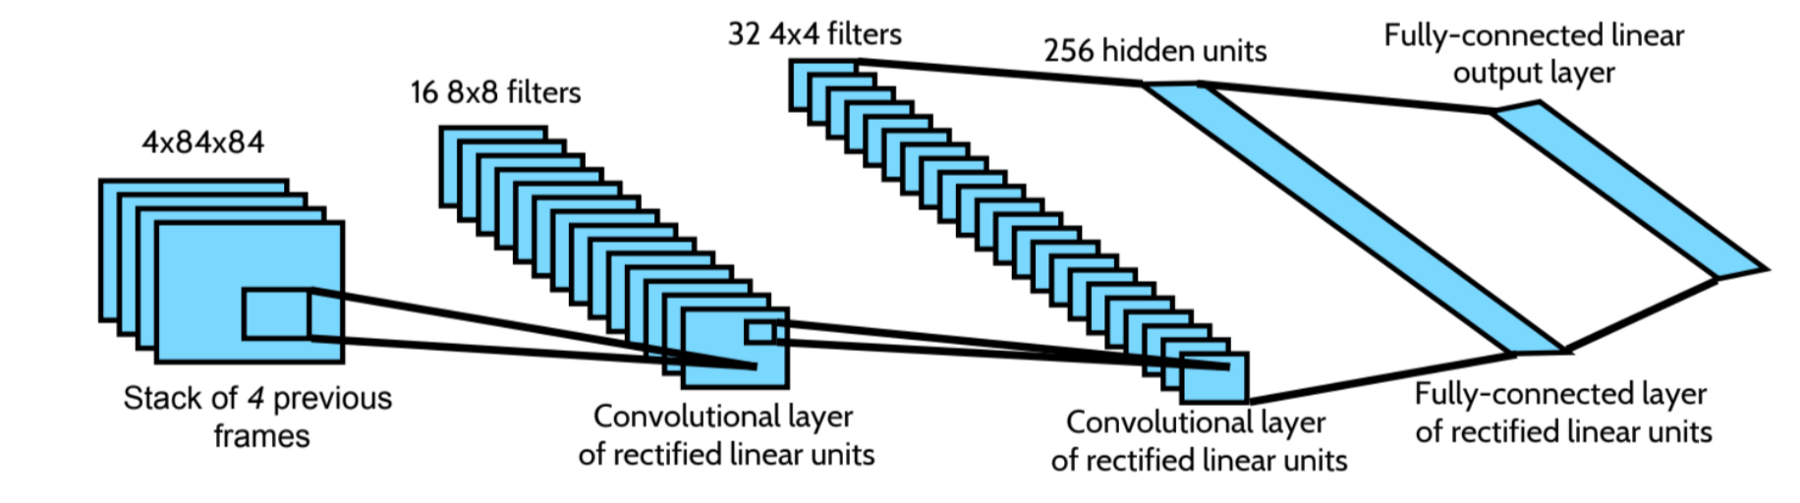
\includegraphics[scale=0.12]{q.png}
\caption{Schematic illustrating neural networks in deep Q learning}
\label{fig:off_control} 
\end{figure}

If the combinations of states and actions are too large, the memory and the computation requirement for Q will be too high. To address that a deep neural network is used to approximate Q(s, a). Such a learning algorithm is called Deep Q-learning (DQN) wherein an input layer takes different representations of the state space, and the output layer predicts Q values for different actions. The action with highest value for Q is chosen with some probability  ($1-\epsilon$), where $\epsilon$ is 1 at the start and reduces to very small values for larger time steps. This is done to take care of the explore-exploit dilemma, so that the agent doesn't stick with a less optimal policy in the begining, and can explore more in the beginning. This is called adaptive $\epsilon$-greedy~\cite{tokic2010adaptive} technique.

\section{Applications}
\label{sec:applications}
 RL has many applications ranging from finance to medicine. In computer vision, for example, RL has been used~\cite{mnih2015human, krull2017poseagent, yun2017action} in such areas as recognition, visual-control, motion-analysis, scene-understanding, etc. RL has been used in the context of personalized medicine and dynamic treatment regime (DTR)~\cite{murphy2003optimal} as well. Another very interesting application of RL was by~\citet{ipek2008self} where the authors propose to design the memory controller (for chip multipro-
cessors (CMPs)) as an RL agent whose goal is to learn automatically an optimal memory scheduling policy via interaction with the rest of the system. 
  

\section{Controlling chaos}
\label{sec:chaos}
Chaotic systems are such non-linear systems which are highly sensitive to initial conditions. Most of the non-linear dynamical systems may become chaotic for some values of the system parameters. Examples include atrial fibrillation in the heart~\cite{garfinkel1997quasiperiodicity} wherein disorganized waves of electrical activity meander through the heart, sometimes lethal; epilepsy in the human brain~\cite{babloyantz1986low}; climate models~\cite{shukla1998predictability}; economics~\cite{vlad2010chaos}, so and so forth. In a way chaos is the rule of nature. Thus controlling chaos to ones advantage is of paramount importance. In this section we illustrate the use of reinforcement learning in controlling chaos. A canonical system, called Lorenz system of equations~\cite{lorenz1995essence}, is used to simulate chaos. The related equations are given as,

\bea
\frac{dx}{dt}&=&\sigma(y-x) \\
\frac{dy}{dt}&=&x(\rho - z) - y \\
\frac{dz}{dt}&=&xy - \beta z
\eea

where $\sigma=10$, $\beta=8/3$, $\rho=28$ are parameters. The solution ([]x,y,z]) of these equations with time is plotted in the 3D plot of figure~\ref{fig:off_control} . Note the butterfly shape of the solution space, and how solution varies chaotically within this butterfly which has limits between -20 to 20.

\begin{figure}[ht!]
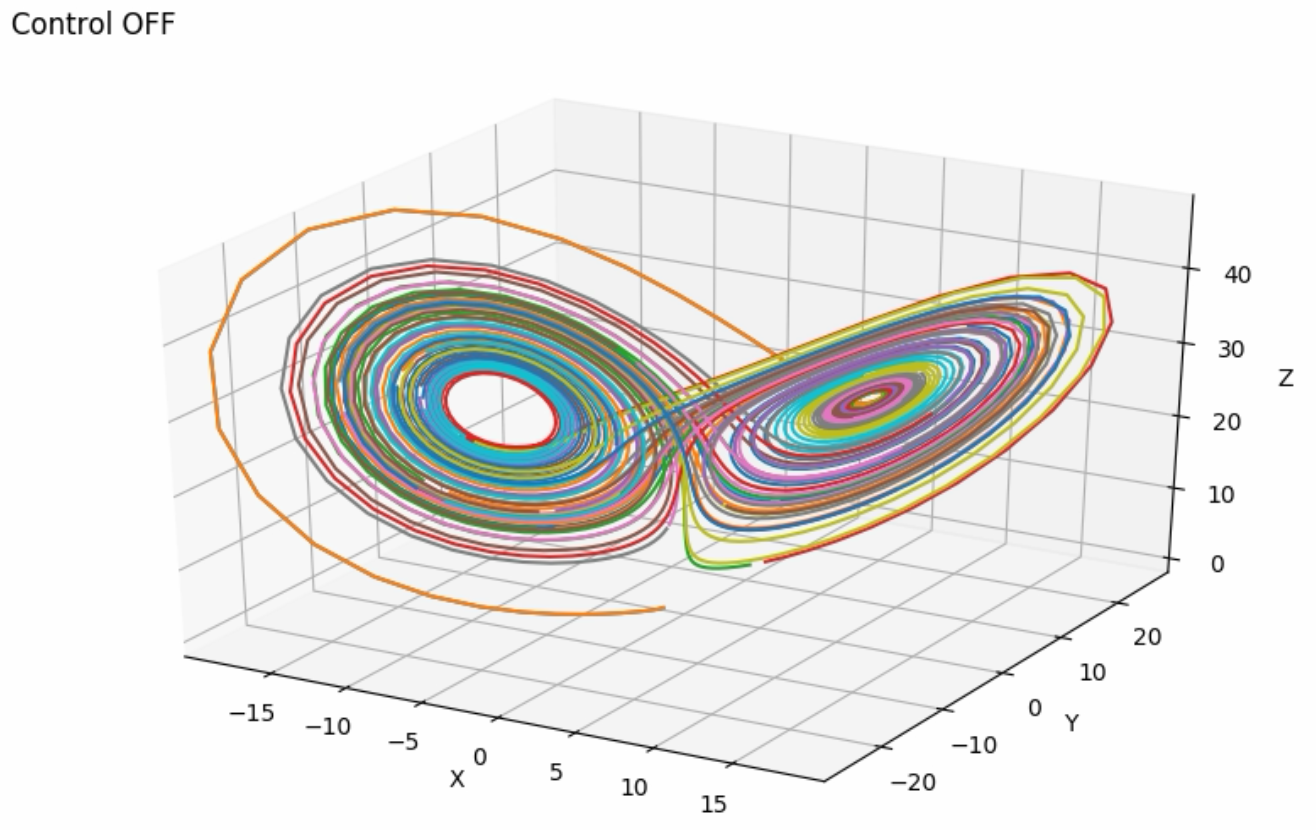
\includegraphics[scale=0.15]{OFF.png}
\caption{Solution of the Lorenz system of equations with time without control}
\label{fig:off_control} 
\end{figure}
We attempt to control this chaotic solution, i.e. confine this solution to a limited region using reinforcement learning. This is done by perturbing the parameters in Eqs.(2,3,4) infinitesimally by $\sigma_p$, $\rho_p$, $\beta_p$ respectively. The resulting equations are,

\bea
\frac{dx}{dt}&=&(\sigma+\sigma_p)(y-x) \\
\frac{dy}{dt}&=&x((\rho + \rho_p) - z) - y \\
\frac{dz}{dt}&=&xy - (\beta + \beta_p)z
\eea

The values of these perturbations are less than 1\% of the original parameters, and are evaluated by the RL agent at every time step such that the solution from these equations never deviates from the specified limit. The state space S for the agent are the position coordinates (x,y,z) and their derivatives ($\frac{dx}{dt}$, $\frac{dy}{dt}$, $\frac{dz}{dt}$); the environment is a continuous space of coordinates (x,y,z), and the action space is the value of the perturbation parameters. The reward function is defined as follows,

\bea
|l_{t+2} - l_{t}| <=1, R =1 \\
|l_{t+2} - l_{t}| >1, R = -1
\eea

where $l_t$ represents the vector (x,y,z) at time t.  The RL based chaos controller is used to confine this solution within a deviation of 2 units, and the resulting solution is plotted in figure \ref{fig:on_control}. 

We use proximal policy optimization (PPO2) from OpenAI stable-baselines~\cite{stable-baselines} with a policy network of two hidden layers (64 hidden units each). The environment for Lorenz system is written in a OpenAI gym~\cite{brockman2016openai} compatible python format.

Note that the solution here is confined to a limited region, thereby limiting the randomness within the solution space. Thus, we say that a control on chaos was attained. Several other control goals such as making the solution to follow a desired orbit in the space, etc, can be attained.

\begin{figure}[ht!]
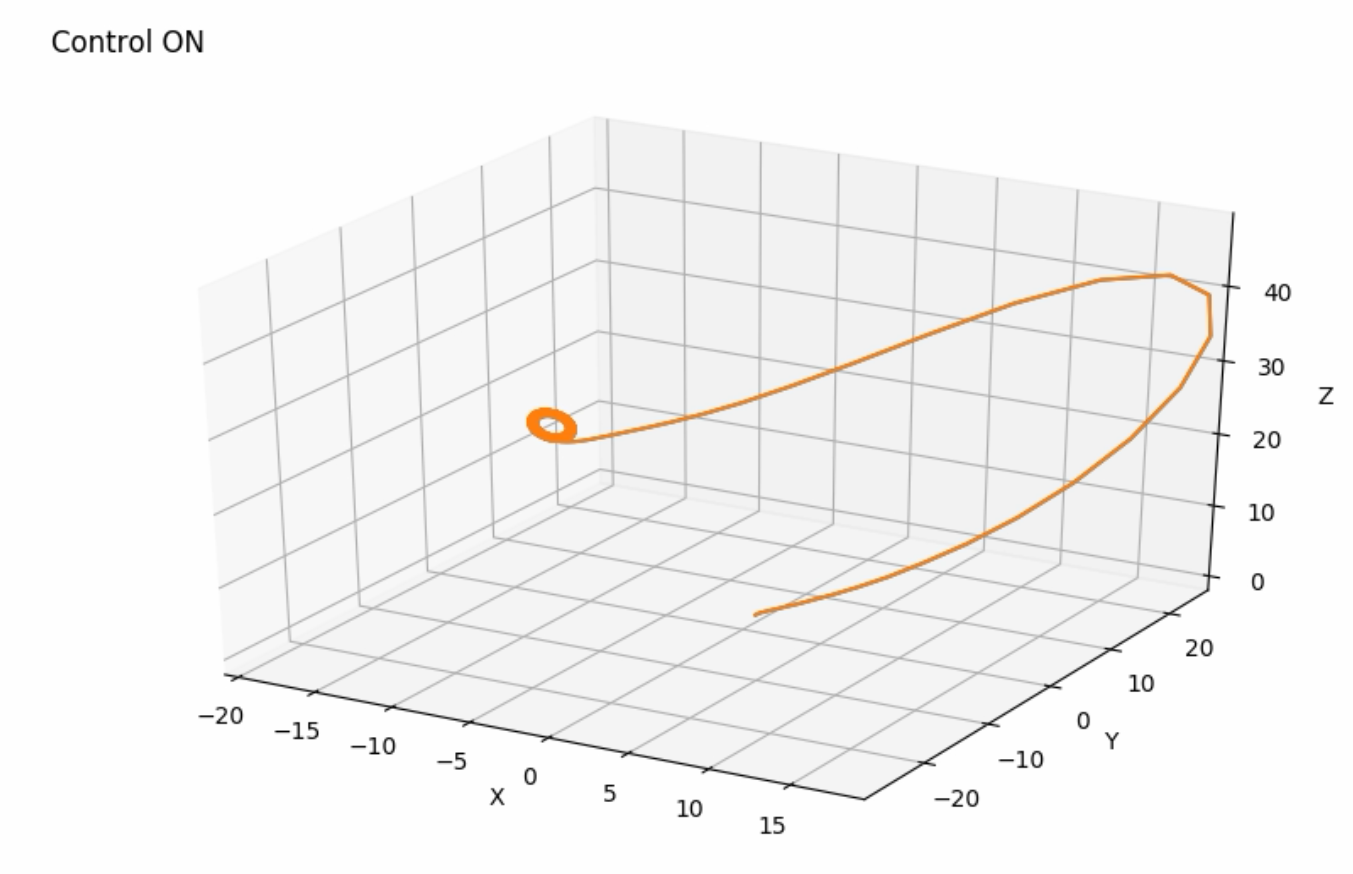
\includegraphics[scale=0.15]{ON.png}
\caption {Solution of the Lorenz system of equations with RL based control. Note that the final solution is confined in a small ring like region, unlike the uncontrolled solution which wanders throughout space; thus the RL based control significantly reduces the randomness in solution. }
\label{fig:on_control} 
\end{figure}


\section{Conclusions}
\label{sec:Conclusion}

%We have provided a basic overview of reinforcement learning in this report. Besides, a deep reinforcement learning based controller for a canonical chaotic system was developed and detailed in this report. The relevant codes, animation have been attached with this pdf.


\section*{Acknowledgments} 
%The authors would like to thank Prof. Oge Marques for being flexible enough in permitting to choose a topic of interest for the final project. 

\bibliography{cov_bib.bib}

  
%\bibliography{journal,book,preprint,report}
%
\end{document}

